% Division with decimals worksheet template
\documentclass[leqno, 12pt]{article}
\usepackage[a4paper, portrait, margin=1cm]{geometry}
\usepackage{amsmath}  % for newcommand
\usepackage{tikz} 
\usetikzlibrary{positioning}
\usepackage{multicol}
\usepackage{fancyhdr}


\newcommand\Mydiv[2]{%
$\strut#1$\kern.25em\smash{\raise.3ex\hbox{$\big)$}}$\mkern-8mu
 \overline{\enspace\strut#2}$}

\def \HeadingQuestions {\section*{\Huge Name: \underline{\hspace{8cm}} \hfill Date: \underline{\hspace{3cm}}}
{Division with decimals: Questions} \vspace{1pt}\hrule}

% raise footer with page number
\fancypagestyle{myfancypagestyle}{
  \fancyhf{} % clear all header and footer fields
  \renewcommand{\headrulewidth}{0pt} % no rule under header
  \fancyfoot[C] {\thepage} \setlength{\footskip}{16pt} % raise page number 6pt
}
\pagestyle{myfancypagestyle}  % apply myfancypagestyle

% 
\begin{document}
    \HeadingQuestions
    \vspace{-5mm}
    \begin{multicols}{2}

        \begin{equation} \begin{tikzpicture}[baseline=(current bounding box.center)] \Mydiv{5}{34.8} \end{tikzpicture} \end{equation}


        \begin{equation} \begin{tikzpicture}[baseline=(current bounding box.north)] \Mydiv{5}{34.8} \end{tikzpicture} \end{equation}

        \begin{equation} \begin{tikzpicture}[baseline=(current bounding box.center)] \Mydiv{5}{34.8} \end{tikzpicture} \end{equation}

        \begin{equation} \begin{tikzpicture}[baseline=(current bounding box.north)] \Mydiv{5}{34.8} \end{tikzpicture} \end{equation}


        \begin{equation}
            \\
            \quad \Mydiv{5}{5415} \quad \\
            \\
        \end{equation}
        \begin{equation}
            \\
            \quad \Mydiv{5}{5415} \quad \\
            \\
        \end{equation}
        \begin{equation}
            \begin{tikzpicture}[baseline={([yshift=-1pt]current bounding box.north)}]
        
            \Mydiv{5}{34.8}\\
        
        \end{tikzpicture}
        \end{equation}
    \end{multicols}
\end{document}
